\chapter{Implementacja}
\label{cha:implementation}

\section{Architektura rozwiązania}

\begin{figure}[!ht]
	\begin{center}
		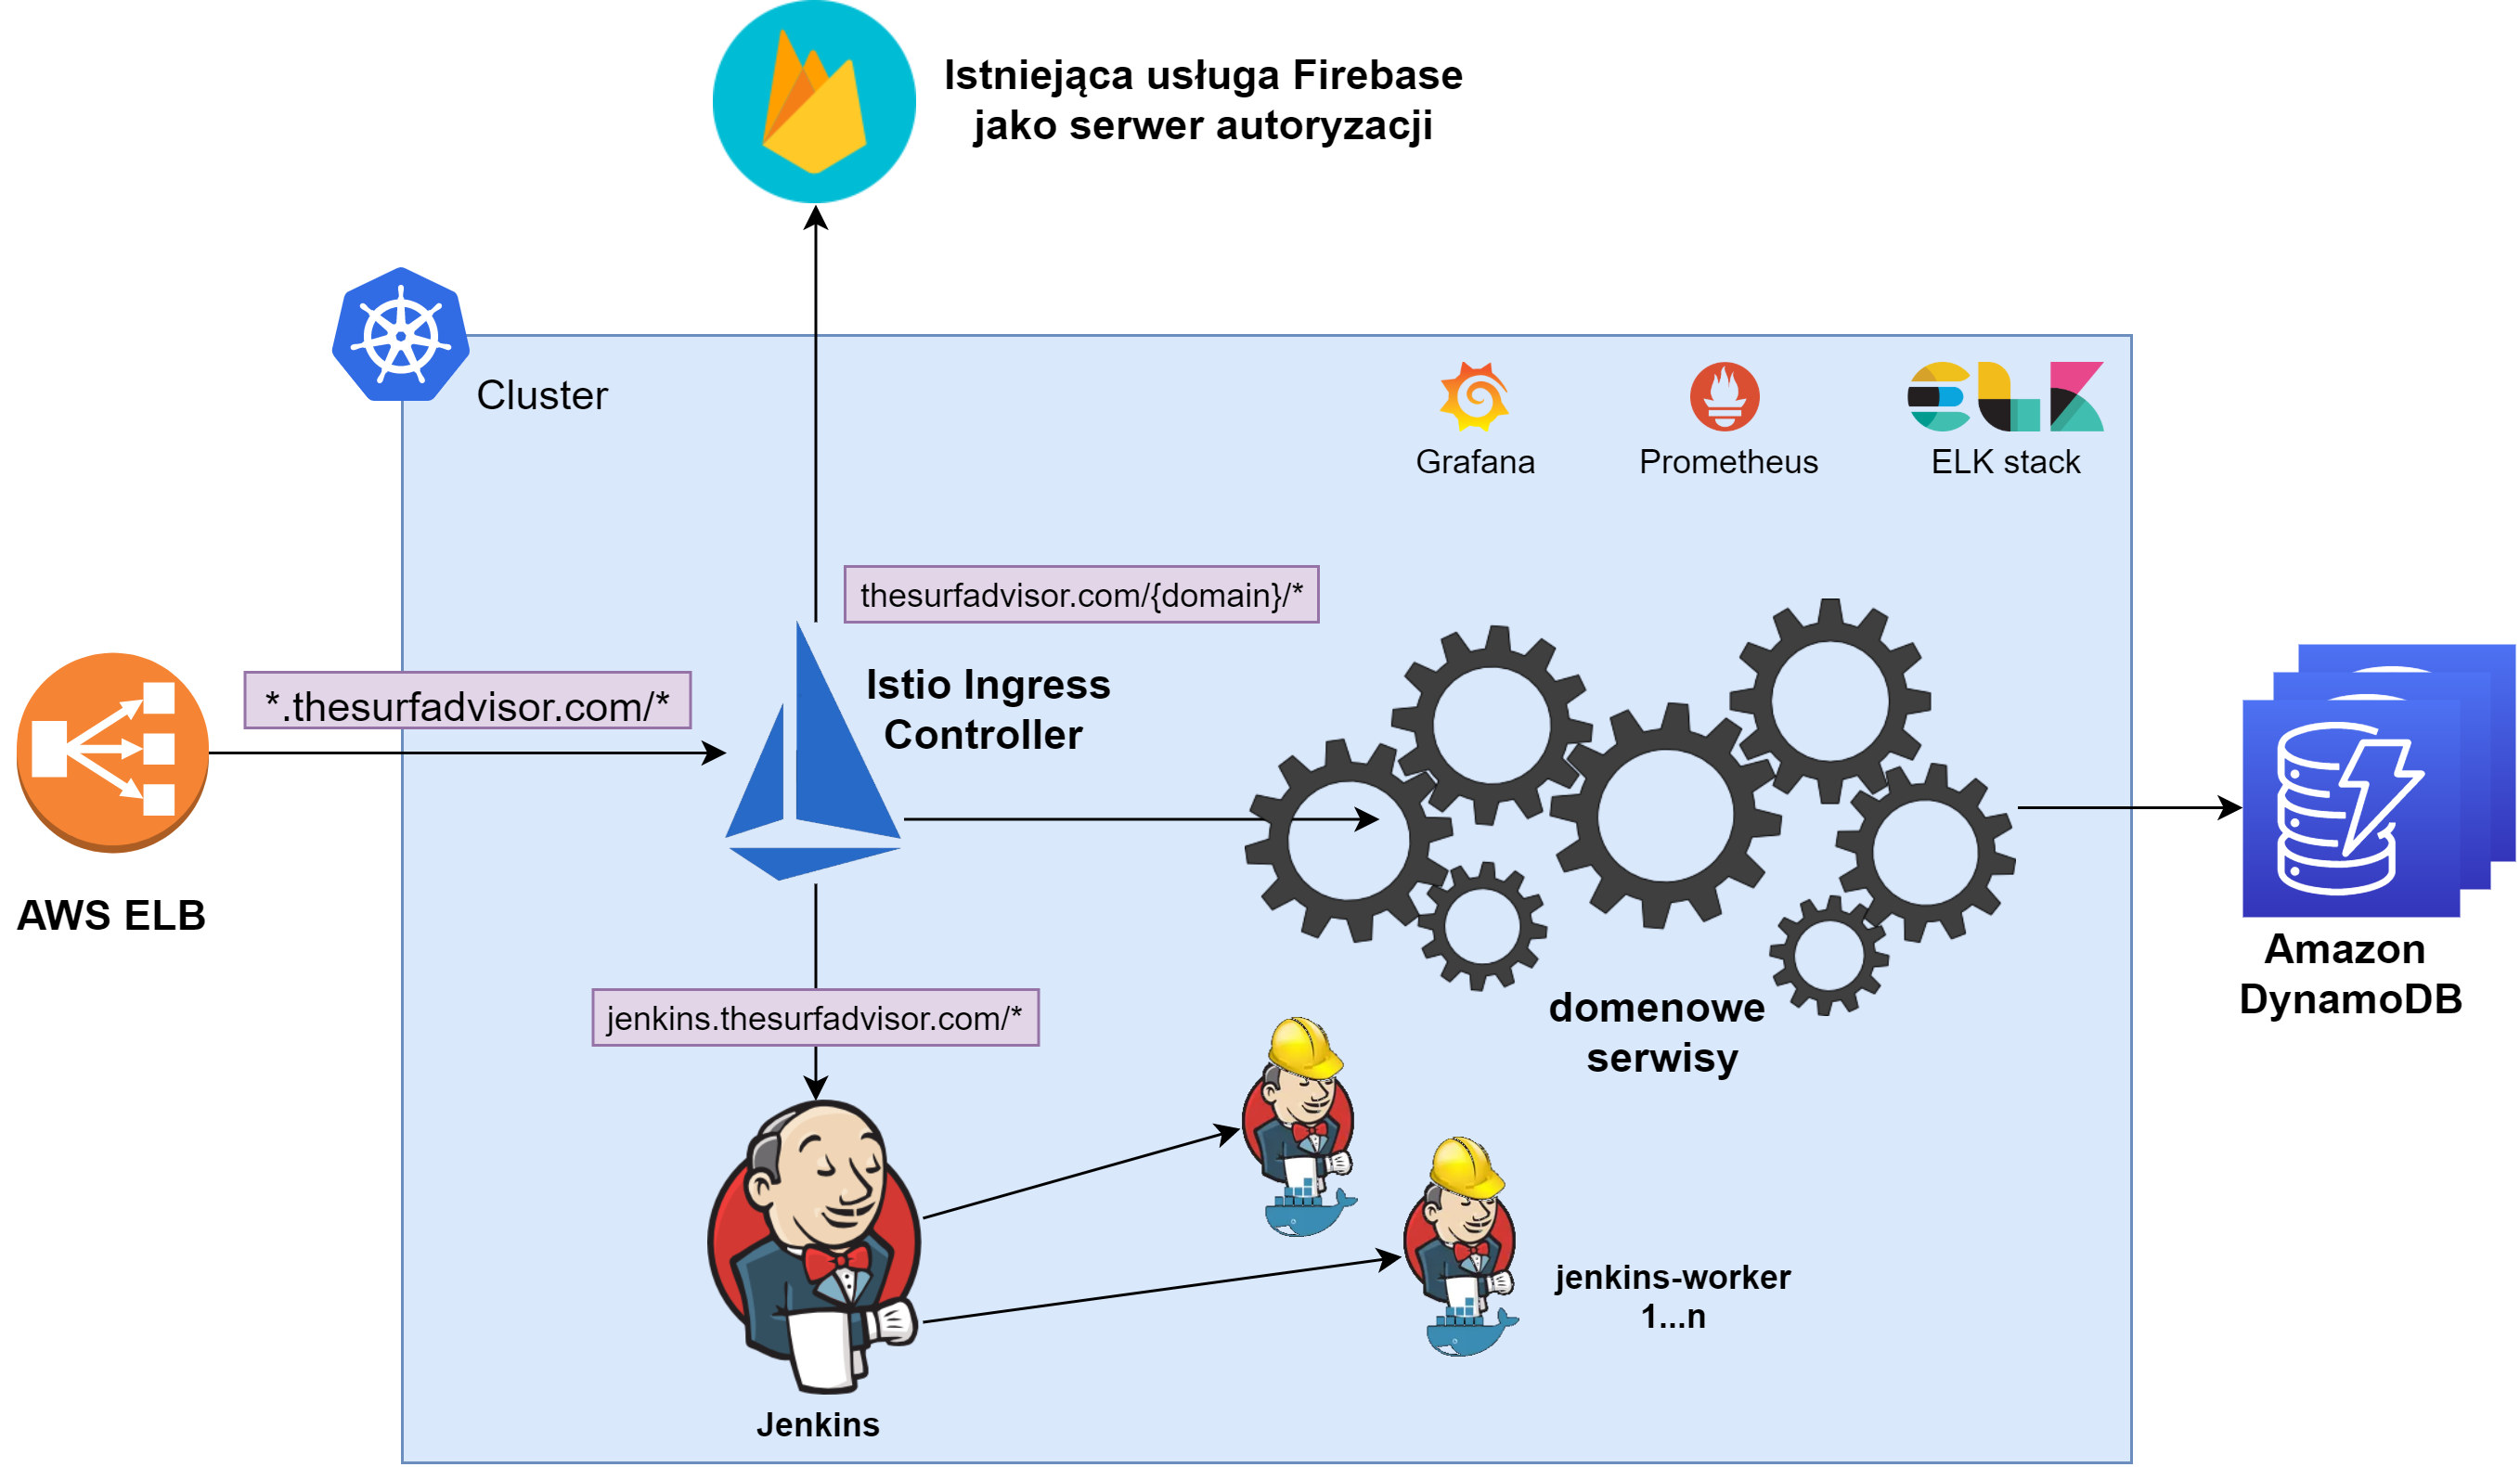
\includegraphics[width=1\textwidth]{img/surf-cluster}
	\end{center}
	\caption{Cluster nowych usług SurfAdvisor}
\end{figure}

\cw{Cluster} nowych usług SurfAdvisor w spoczynku składa się z: 

\begin{itemize}
    \item
    1 x master \cw{Node} - EC2 \textbf{m3.medium} \emph{(1 vCPU \& 3.75 GiB RAM)}

    \item
    2 x worker \cw{Node} - EC2 \textbf{t3.medium} \emph{(2 vCPU \& 4 GiB RAM)}
\end{itemize} 

W przypadku zwiększenia natężenia ruchu liczba \cw{Node}'ów jest skalowana by sprostać wymaganiom.
Pod globalnie dostępną domeną \textbf{thesurfadvisor.com} kryje się \emph{Load Balancer} utrzymywany przez AWS.
Stanowi on jedyny punkt dostępu, cały ruch jest następnie obsługiwany przez Istio \emph{Ingress Controller}.
Autoryzacja zintegrowana jest z istniejącym systemem Firebase. Każdy domenowy serwis uderza do własnej bazy danych DynamoDB.

Jako administrator możemy się dostać do subdomen takich jak:

\begin{itemize}
    \item
    \emph{\textbf{jenkins}.thesurfadvisor.com}\\ 
    Jenkins \emph{WEB UI} pracującego wewnątrz \cw{Cluster}'a

    \item
    \emph{\textbf{grafana}.thesurfadvisor.com}\\
    Grafana \emph{WEB UI} śledząca metryki stanu technicznego

    \item
    \emph{\textbf{kibana}.thesurfadvisor.com}\\
    Kibana \emph{WEB UI} do wygodnego przeszukiwania logów
\end{itemize} 



\section{Aplikacje biznesowe}

\begin{figure}[!ht]
	\begin{center}
		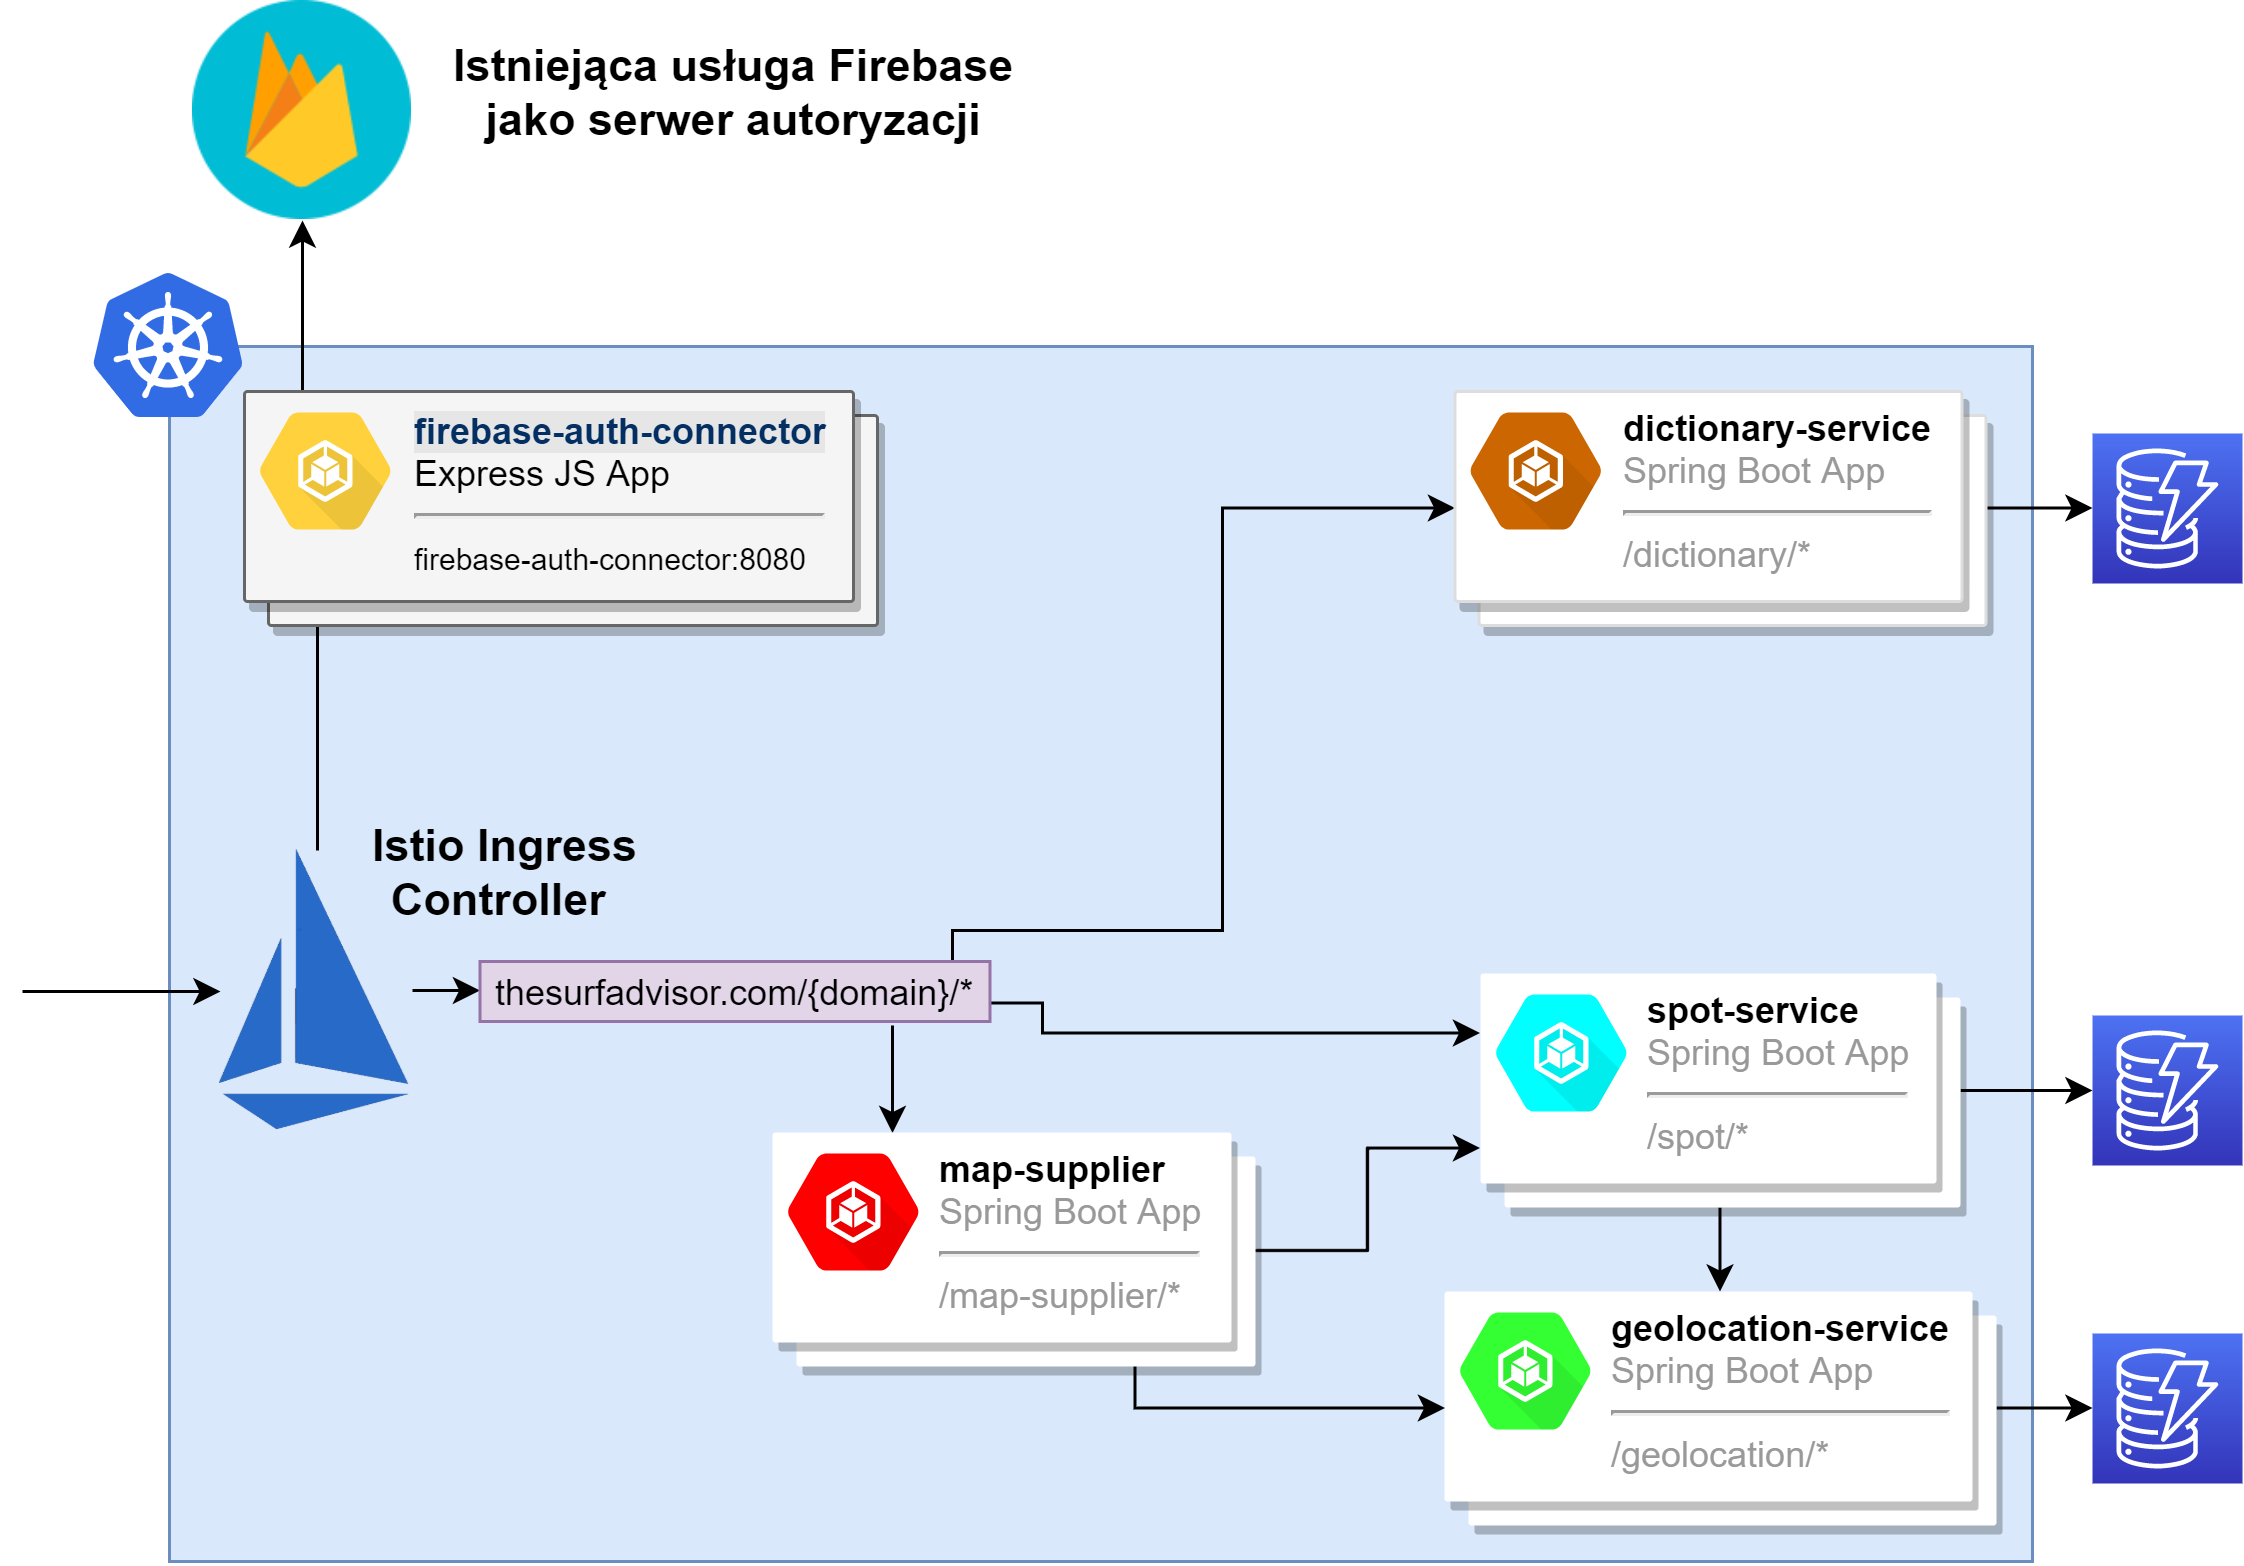
\includegraphics[width=1\textwidth]{img/surf-services}
	\end{center}
	\caption{Zbliżenie na domenowe serwisy SurfAdvisor}
\end{figure}

\begin{itemize}
    \item
    \textbf{firebase-auth-connector}\\ 
    Warstwa pośrednia pomiędzy Istio \emph{Ingress Controller} a istniejącym serwisem Firebase.
    

    \item
    \textbf{dictionary-service}\\ 
    Repozytorium literałów wyświetlanych w aplikacji mobilnej.

    \item
    \textbf{geolocation-service}\\ 
    Wiedza o położeniu obiektów na kuli ziemskiej.

    \item
    \textbf{spot-service}\\ 
    Atlas spotów - miejsc do uprawiania sportu wodnego.

    \item
    \textbf{map-supplier}\\ 
    Agreguje resztę serwisów związanych z mapą, by wydajniej obsłużyć aplikacje mobilną.
\end{itemize} 





\section{IaC - Infrastructure as Code}

(3-5s) jak ja to realizuję w projekcie poprzez CloudFormation, Kubernetes i Jenkins

\subsection{CloudFormation}

\begin{figure}[!ht]
	\begin{center}
		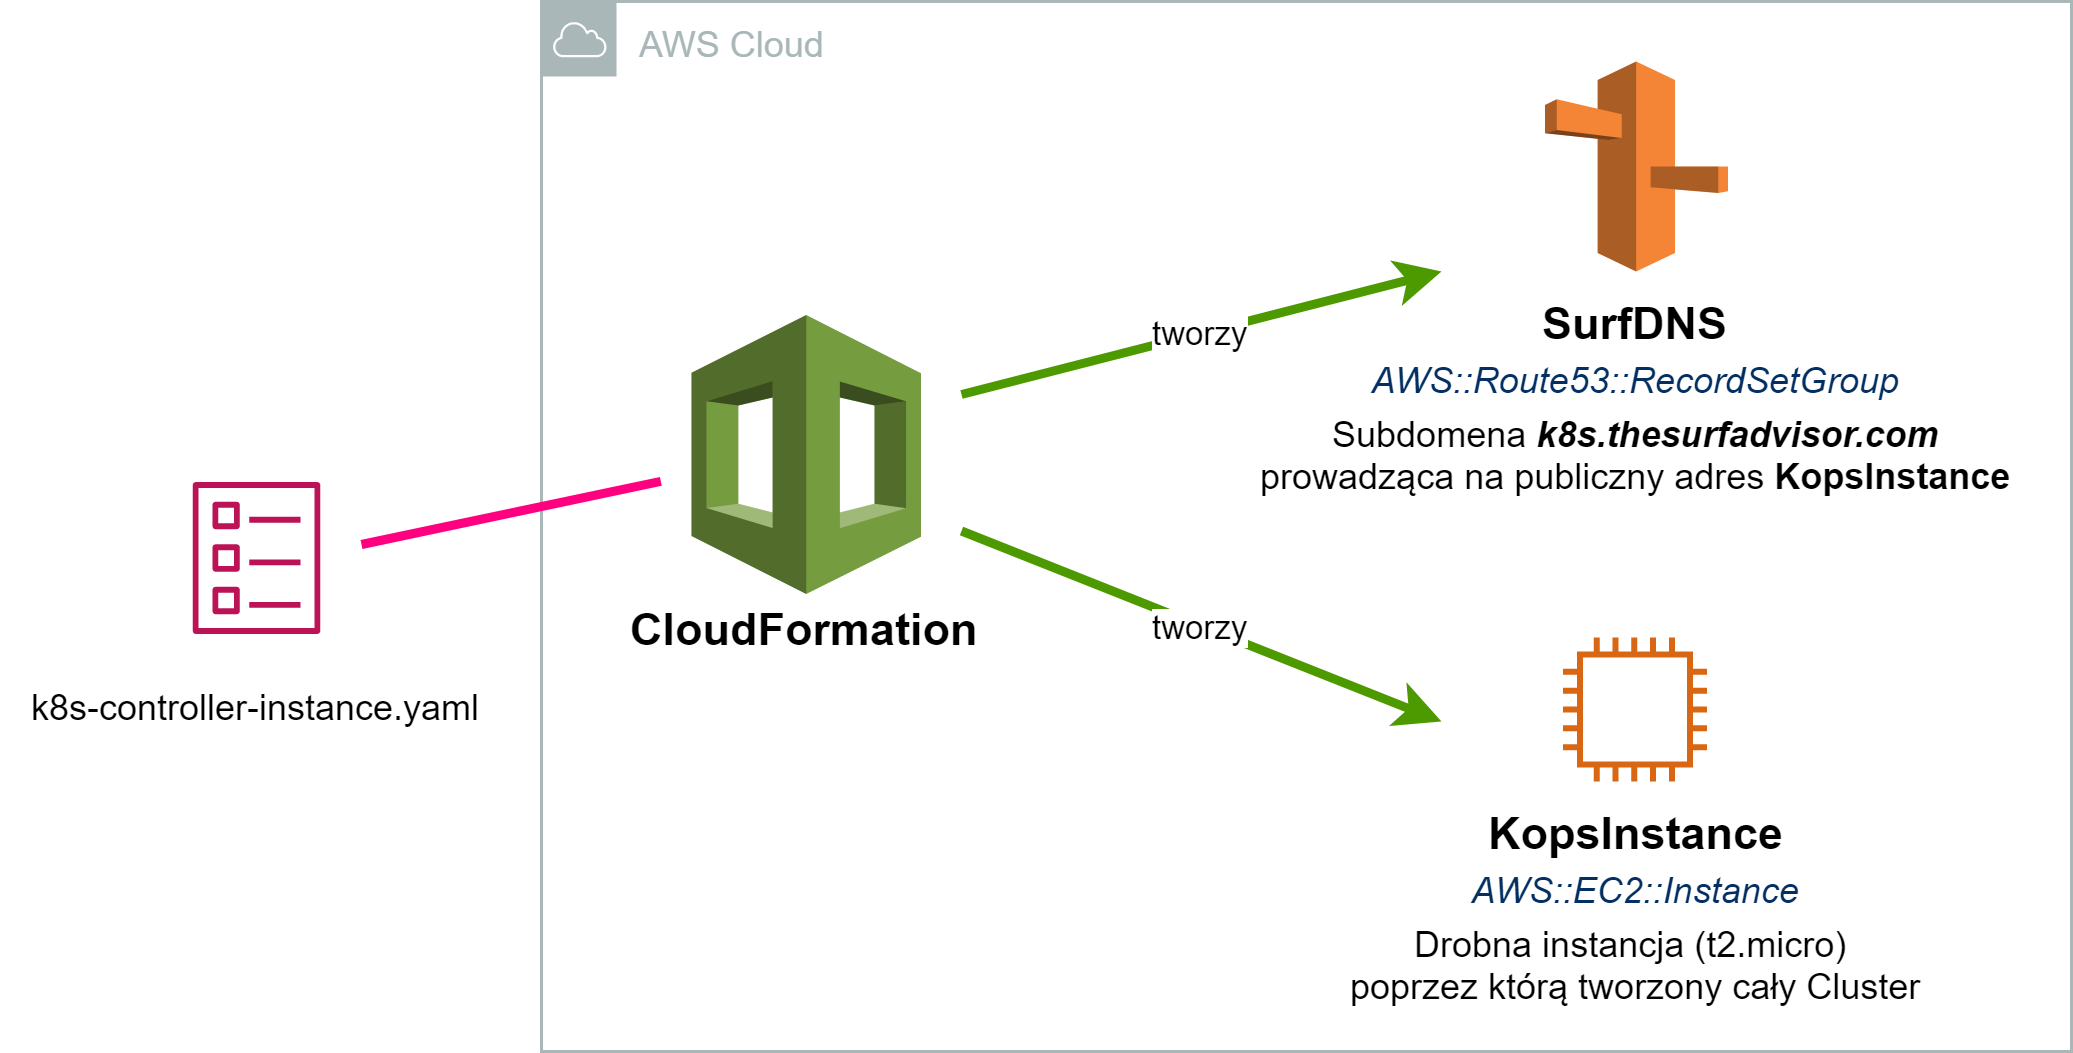
\includegraphics[width=1\textwidth]{img/IAC-step1}
	\end{center}
	\caption{Inicjacja Cluter'a SurfAdvisor - 1.CloudFormation}
\end{figure}

\subsection{Kops}

\begin{figure}[!ht]
	\begin{center}
		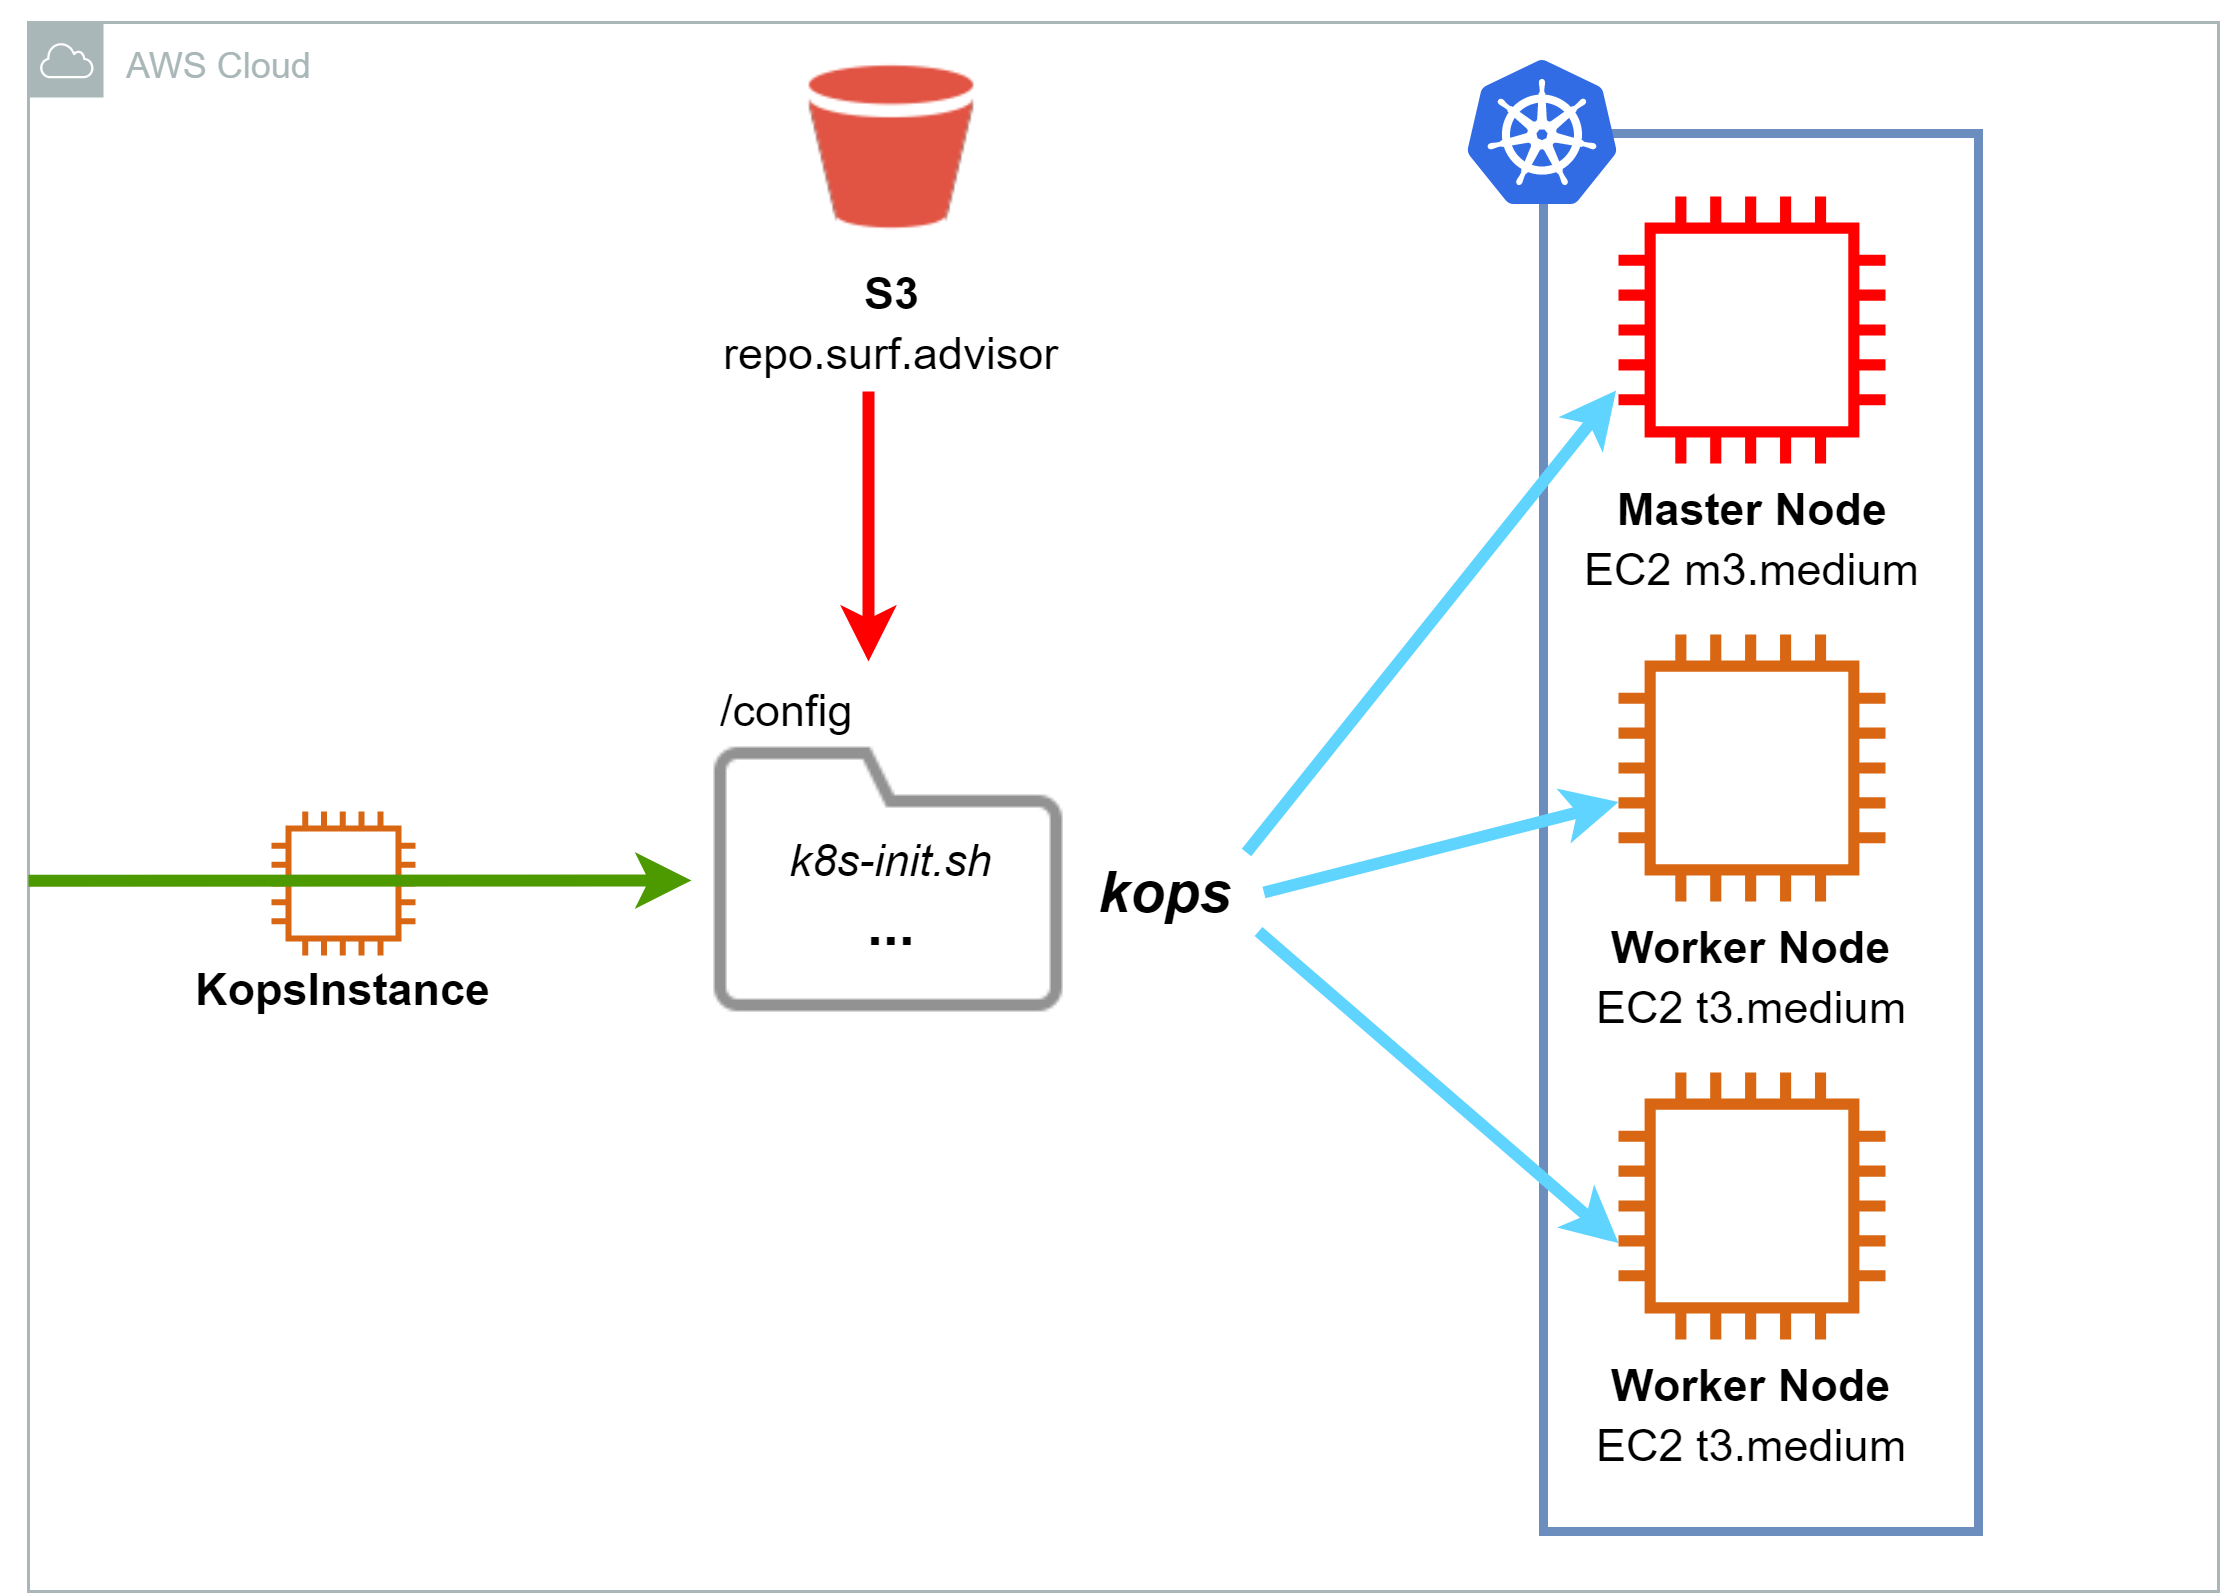
\includegraphics[width=1\textwidth]{img/IAC-step2}
	\end{center}
	\caption{Inicjacja Cluter'a SurfAdvisor - 2.Kops}
\end{figure}

\subsection{Kubernetes}

\begin{figure}[!ht]
	\begin{center}
		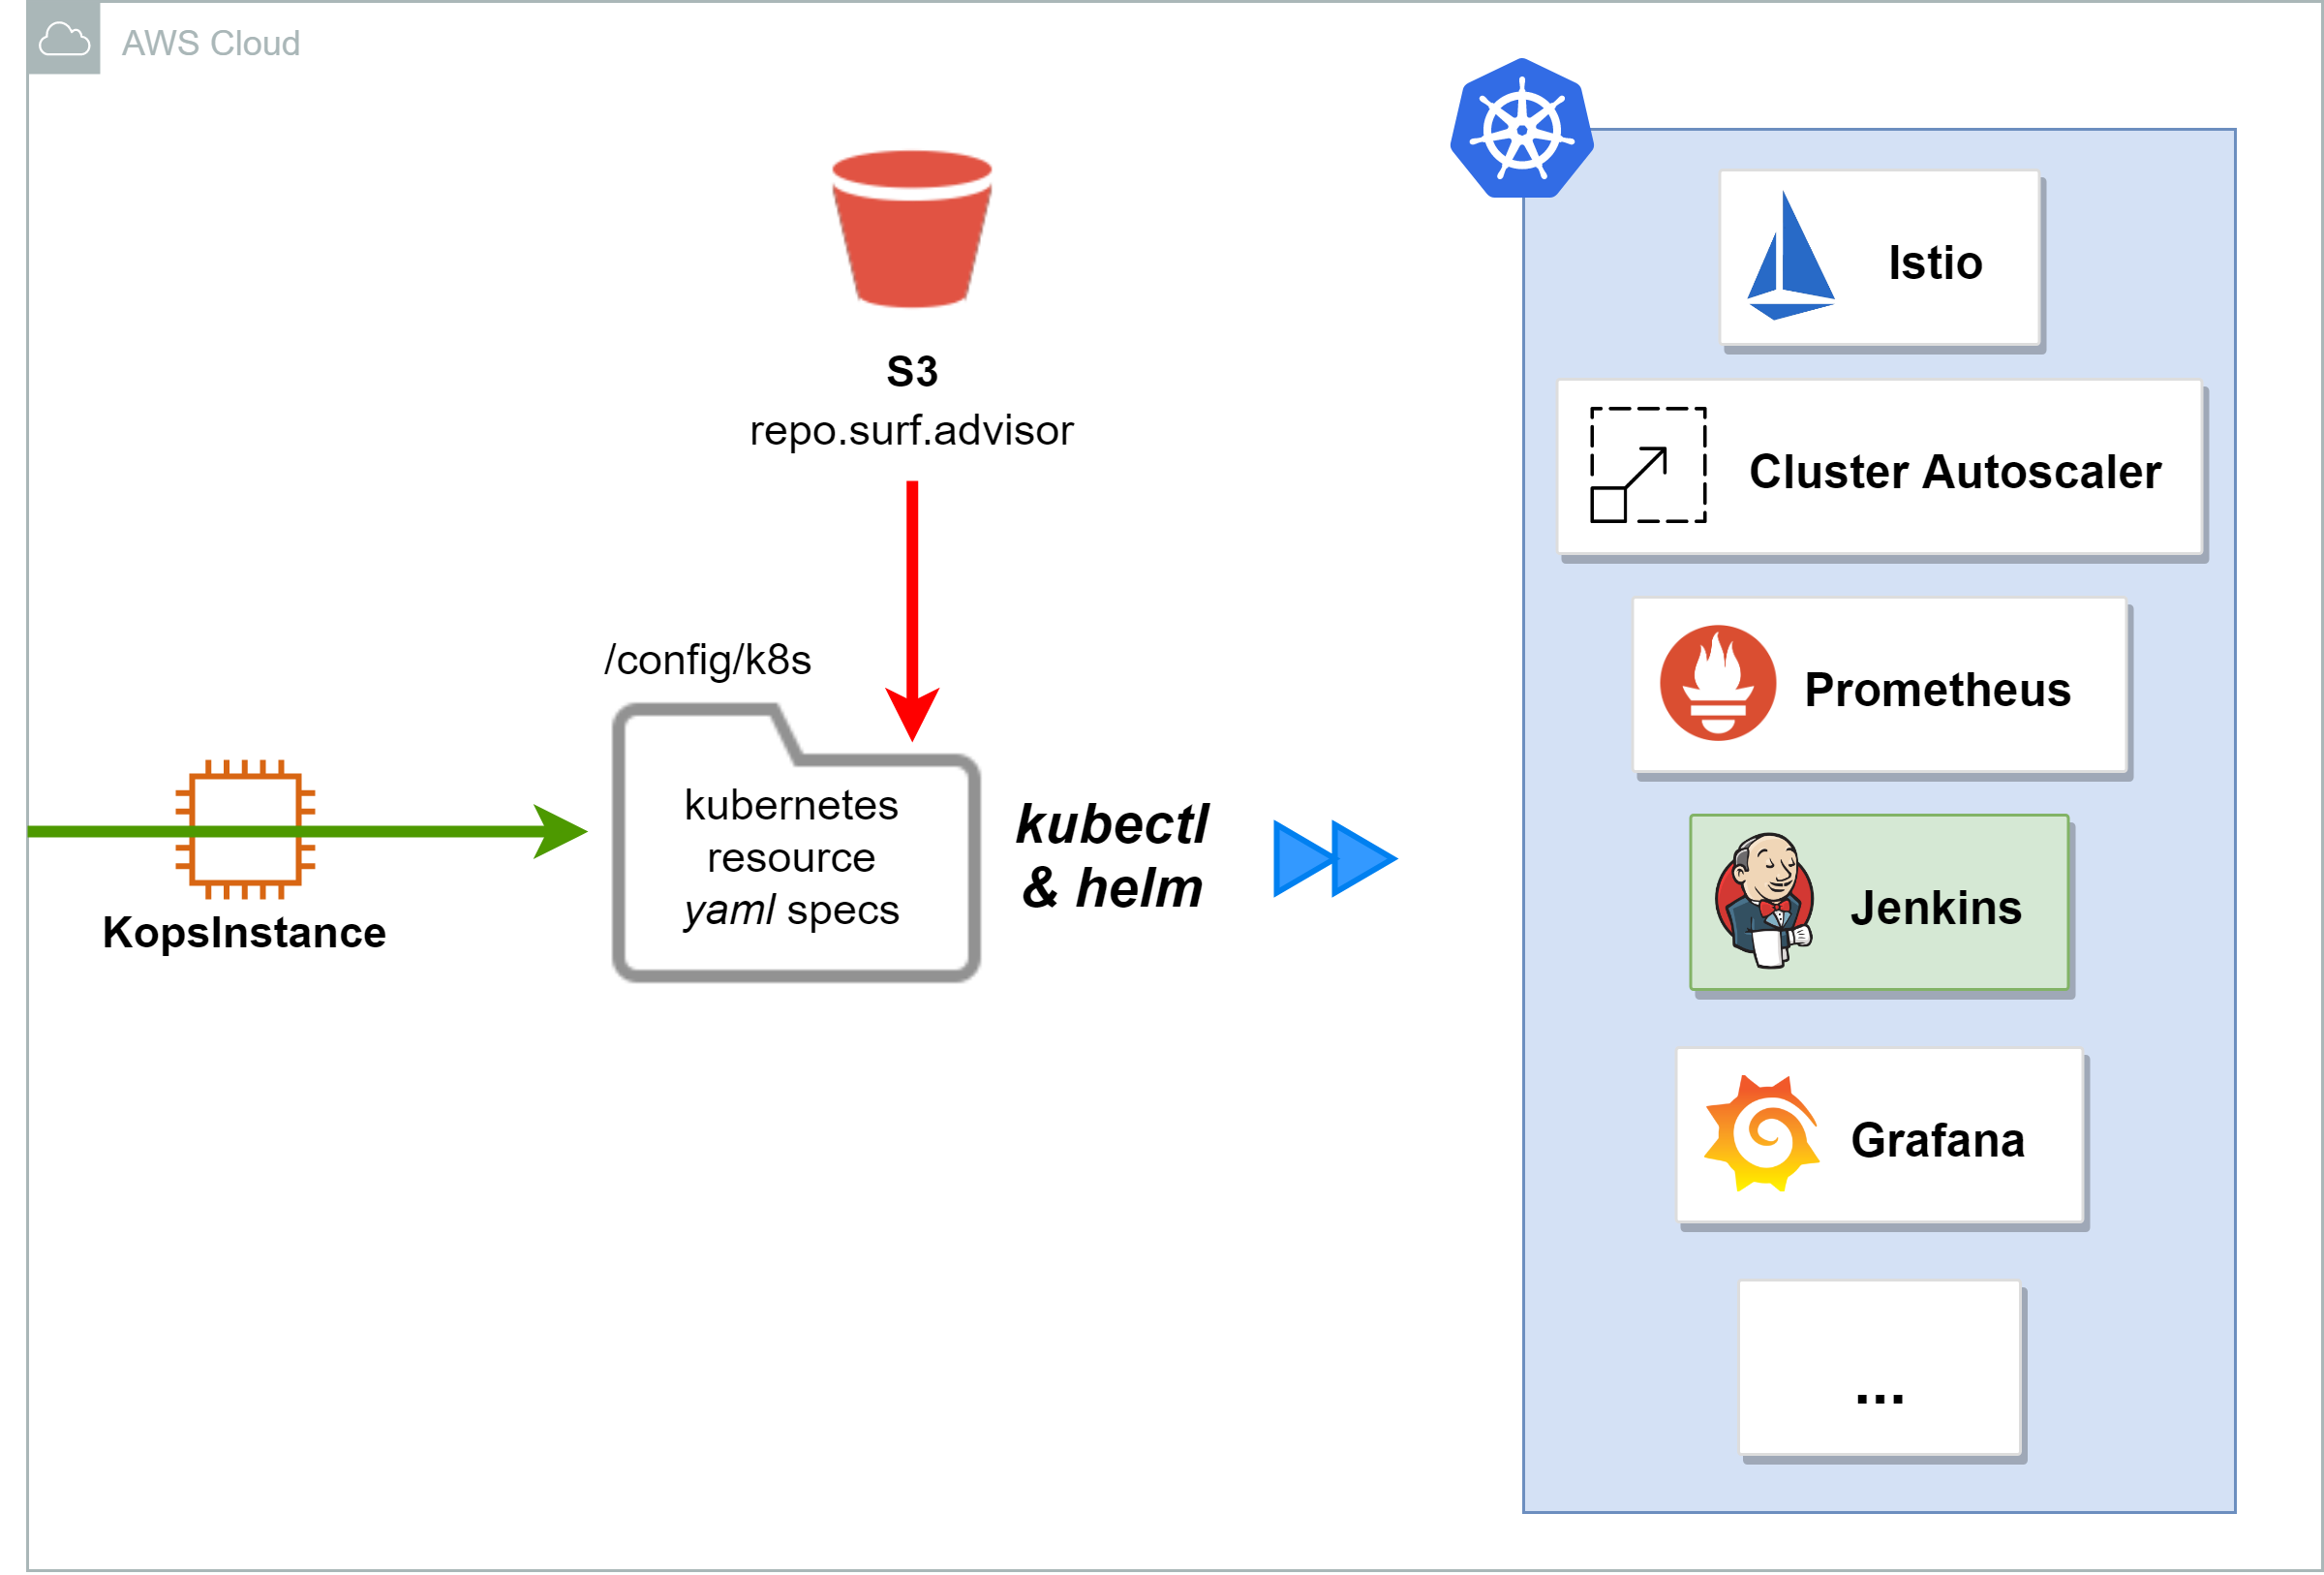
\includegraphics[width=1\textwidth]{img/IAC-step3}
	\end{center}
	\caption{Inicjacja Cluter'a SurfAdvisor - 3.Kubernetes}
\end{figure}

\subsection{Jenkins}

\begin{figure}[!ht]
	\begin{center}
		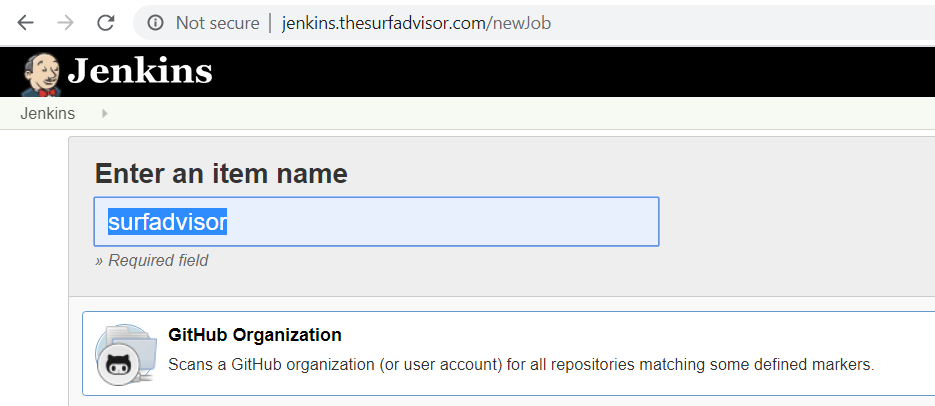
\includegraphics[width=0.8\textwidth]{img/jenkins-new-job}
	\end{center}
	\caption{Jenkins: wdrożenie domenowych serwisów - job "Github Organization"}
\end{figure}

\begin{figure}[!ht]
	\begin{center}
		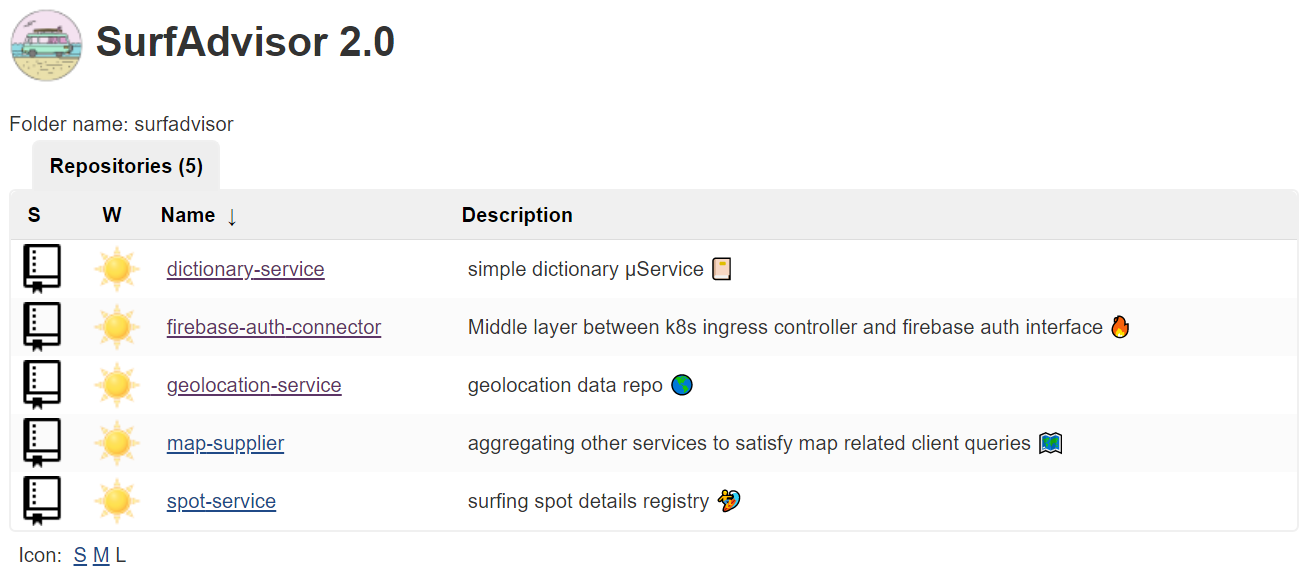
\includegraphics[width=1\textwidth]{img/jenkins-surf-folder}
	\end{center}
	\caption{Jenkins: wdrożenie domenowych serwisów - folder SurfAdvisor}
\end{figure}

\begin{figure}[!ht]
	\begin{center}
		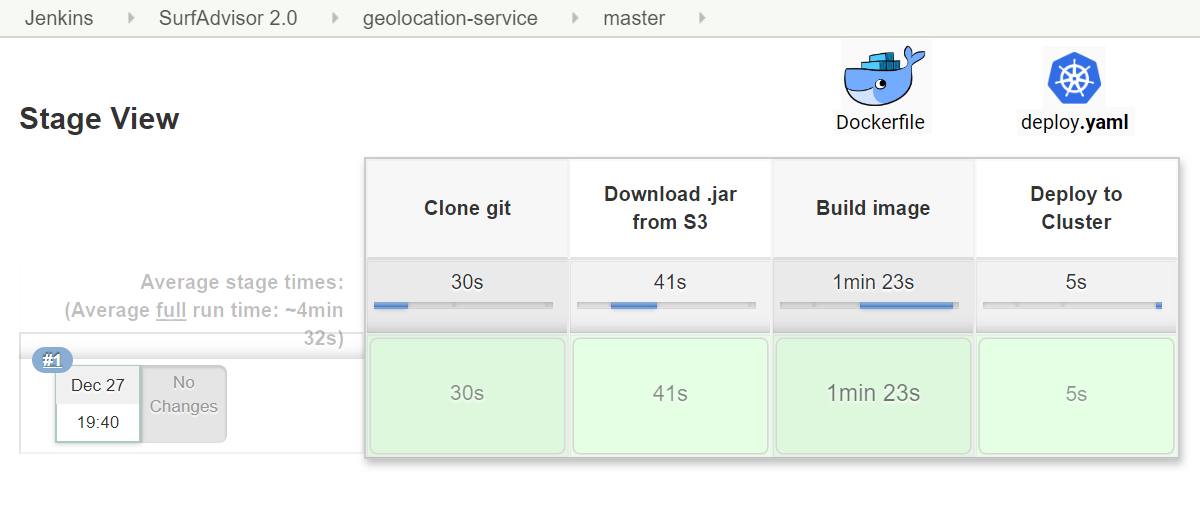
\includegraphics[width=1\textwidth]{img/jenkins-geo-stages}
	\end{center}
	\caption{Jenkins: wdrożenie domenowych serwisów - pipeline}
\end{figure}



 

\section{Zarządzanie ruchem}
(2-3s) o rutowaniu i security

\section{Monitoring}
(1-2s) obserwacja parametrów technicznych przy użyciu Prometheus \& Grafana


\section{Realizacja wymagań funkcjonalnych}
(5-10s) Geohash \& Clustering + gdzie i jak to implementuję 
- pochylenie się nad serwisami: geolocation-service, spot-service, map-supplier. 
Prezentacja aplikacji mobilnej